\documentclass[12 pt]{article}
\usepackage{hyperref, fancyhdr, setspace, enumerate, amsmath,
  lastpage, amssymb}
\usepackage[margin=1 in]{geometry}
\allowdisplaybreaks
%\usepackage[dvipsnames]{xcolor}   %May be necessary if you want to color links
\hypersetup{
	%colorlinks=true, %set true if you want colored links
	linktoc=all,     %set to all if you want both sections and subsections linked
	linkcolor=black,  %choose some color if you want links to stand out
}
\usepackage{graphicx}
\graphicspath{{Images/}}
% Independent symbol
\newcommand\independent{\protect\mathpalette{\protect\independenT}{\perp}}
\def\independenT#1#2{\mathrel{\rlap{$#1#2$}\mkern2mu{#1#2}}}
\author{Julian Lore}
\date{Last updated: \today}
\title{MATH 324: Statistics}
\pagestyle{fancy}
\lhead{MATH 324}
\chead{\leftmark}
\rhead{Julian Lore}
\cfoot{Page \thepage \ of \pageref{LastPage}}
\newcommand{\tab}[1]{\hspace{.2\textwidth}\rlap{#1}}
\begin{document}
	\onehalfspacing
	\maketitle
	Notes from Masoud Asgharian's Winter 2018 lectures.
	\tableofcontents
        \section{01/09/18}
        \paragraph{What we will cover this semester}
        Will essentially cover chapter 8,9,10. For chapter 11, he will
        give us his own notes. The first 6 sections of chapter 13 and
        a few sections from chapter 14. Occasionally we will go back
        to chapter 7 to revisit things like the t distribution.
        \\ In 323, we made probabilistic models. Statistics is the
        breach in which we connect these models to real
        life. Otherwise, those are just models. A core part of data
        analysis and data sciences is statistics and computer
        science.
        \subsection{Overview - What is Statistics?}
        Inductive logic, we have a sample from the population we want
        to make inference about. With this data, we want to extend the
        results to the whole population. From small to large, sample
        to the population.
        % Image
        \\ 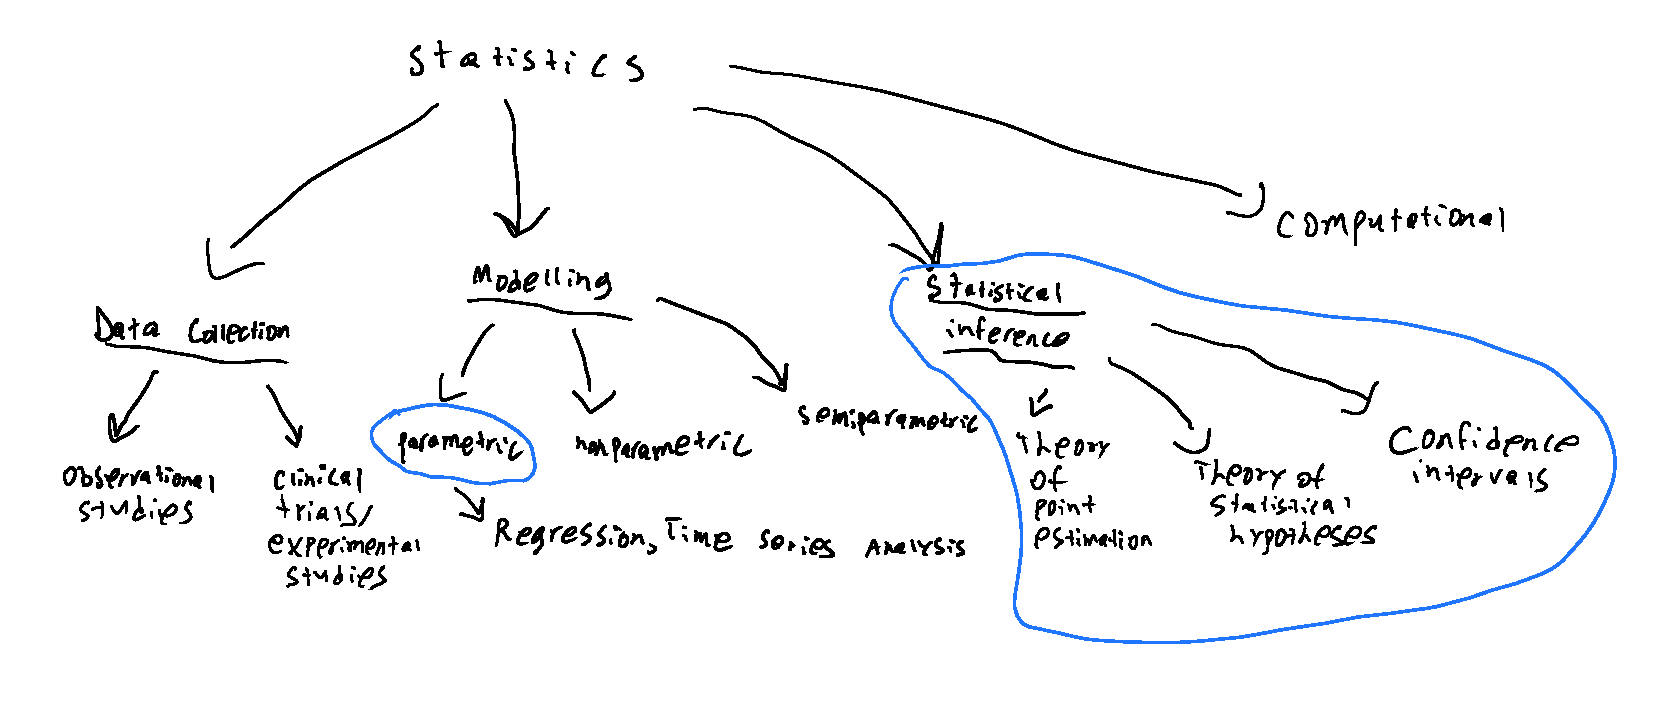
\includegraphics[width=\textwidth]{i1.pdf}
        \begin{itemize}
        \item Observational studies: we go to the population and make
          observations.
        \item Experimental studies: give test subjects something,
          i.e. give them cigarettes when trying to test for if
          cigarettes lead to cancer. Need
          to account for causation, other factors that can affect
          outcome. In order to do so we have to keep their diet and
          other factors controlled. We must also have some sort of
          randomization, we can't send all males to one group and all
          females to another, as males may have a tendency to smoke or
          something of the like. These are also called clinical
          trials.
        \item When we have data, the next step is modeling. May
          occasionally speak of this, but this is not part of the
          course. There are different approaches to modeling, can be
          split into 3 parts.
          \begin{itemize}
          \item Parametric: the salary is distributed like a
            distribution (ex. Gamma), but we don't know the
            parameters. Take for example, we always know that the
            normal distribution is a bell curve, but we don't know
            where it's centered. Very useful, but we might have a
            miss-specification. How do we know our models are correct?
            Most of the time we will be talking about
            \textbf{parametric} models.
          \item Semiparametric
          \item Nonparametric: since we don't know if parametric
            models are correct, we make no assumption about the
            distribution. We just assume that $X \sim F$, all we
            assume about $F$ is that it's continuous, nothing
            more. This is an infinite dimensional vector. Why? How do
            we know a function? We have a vector for $F$, like
            $F(1),F(2, \ldots)$. How do we approximate this? $X_i
            \stackrel{iid}{\sim}F, i=1,2,\ldots,n$. $n$ patients, with
            all the same distribution. So $F(t)=P(X\leq t)$. What does
            this tell us? The proportion of time that $x$ falls below
            $t$. So with $n$ samples, how do we mimic this? We count
            the number of observations below $t$, i.e. $\frac{\#X_i
              \leq t}{n}$, which is an approximation of the
            above. This is an empirical observation. More
            mathematically:
            \begin{equation*}
              \varepsilon(t) =
              \begin{cases}
                1 & \text{if }t\geq 0
                \\ 0 & \text{otherwise}
              \end{cases}
            \end{equation*}
          So we have
          $\hat{F}_n(t)=\frac{1}{n}\sum_{i=1}^n\varepsilon(t-x_i)$. This
          gives us a binomial distribution. But we are assuming they
          are all the same distribution.
          \\ Nonparametric approaches are good for functions of single
          variables, but not for multi variables, which is what
          semiparametric was made for.
          \end{itemize}
          \item Bayesian inference: when you learn that $X \sim N(\mu,
            \sigma^2)$, $X$ is normally distributed and $\mu$ is the
            average of the whole population. Bayes' approach says that
            these parameters are not constants, these are random
            variables themselves. Bayes did not look at probability as
            a frequentest approach, not the proportion of when something
            arrives (frequentest approach works when we have a huge
            sample). The other approach that Bayes had was an updating
            approach, that our parameters are unknown. This is good
            for when you have a stream of data (machine learning is a
            prime example). We have a lack of knowledge and then we
            update it using Bayesian's approach. $\to X | \mu,
            \sigma^2 \sim N (\mu, \sigma^2)$, i.e. the parameters are
            also normally distributed.
          \end{itemize}
          Most of the time we'll be at parametric modeling and
          statistical inference.
        \subsection{Point Estimation} What do we mean by point
        estimation? A scientific guess about the unknown parameter of
        the population. Consider the following situation:
        \\ $x_1, \ldots, x_n \sim N(\mu, 1)$ (usually interested in
        the normal distribution, binomial and poisson). Suppose this
        is the IQ of high school graduates in Canada (the $X_i$ are
        numbers). Why do we call this distribution normal? Because for
        a healthy population, most of the weight should be in the
        middle, just like the bell curve. The Normal distribution is
        especially important for modeling error. For insurance
        companies, we see at the tails that there aren't many large
        claims.
        \\ We want to find $\mu$. Recall that $E(X_i)=\mu,
        i=1,2,\ldots,n$ (if they all have the same observations, they
        have the same mean).
        \\ First, what is a point estimation? What properties should
        it have? If we know the value of $\mu$, we have the whole
        thing, can calculate everything. How do we estimate this? The
        whole population is huge, so we take a sample part of the
        population, mimicking the real $\mu$, getting $\overline{X}_n
        = \frac{1}{n}\sum_{i=1}^nX_i$. $\overline{X}_n$ is useful, but
        $\overline{X}_n-\mu$ isn't, as there's an unknown we have
        here.
        \paragraph{Statistic} A function of observations that does not
        depend on any unknown parameter.
        \subparagraph{Ex} $\overline{X}_n$ is a
        statistic. $\overline{X}_n - \mu$ is not.
        \paragraph{Estimator} A statistic that aims at estimating an
        unknown parameter (we want to work with it). For example, if
        $\mu$ moves from $-\infty$ to $\infty$, we want to have an
        estimator that also has the same range, not one that is
        strictly positive. Example: $\overline{X}_n$ is an
        estimator. However, consider:
        $$S^2 = \frac{1}{n-1}\sum_{i=1}^n(X_i-\overline{X}_n)^2$$
        This is a statistic, but not an estimator, it always returns a
        positive value. Also, take for example in physics, where each
        measure has a unit of measurement. This statistic wouldn't
        even be the same unit, so it once again is a bad estimator.
        \\ When we take a mean and try to estimate it, the next step
        is to figure out how we quantify possible bias.
        \\ \rule{\textwidth}{0.5 pt}
        $$\varepsilon = |\overline{X}_n-\mu |$$
        We can use Tchbycshev's inequality to put a bound on the
        error.
        \begin{flalign*}
        P(|X-\underbrace{E(X)}_{\mu_x}|>k\sqrt{\underbrace{Var(X)}_{\sigma_x^2}})
        \\ P(|X-\mu_x>k\sigma_x) \leq \frac{1}{k^2}
        \end{flalign*}
        Very useful, assume very little but get lots of
        information. One of the big hammers of probability and
        statistics. The only thing we assume here is the existence of
        the second moment.\\
        Consider $k=3$.
        \begin{flalign*}
          P(|X-\mu_x|>3\sigma_x)\leq \frac{1}{9}
          \\ P(|X-\mu_x|\leq 3 \sigma_x)\geq 1 - \frac{1}{9}\approx \%89
        \end{flalign*}
        Without knowing anything else about the distribution, this
        tells us that about $89\%$ of the population is within $3$
        times the variance of the mean.
        \section{01/11/18}
        Last lecture we learned about statistics, estimators and how
        we can measure deviation from the target and the estimation.
        \\ We had $n$ random variables: $x_1, \ldots, x_n, \mu
        \rightarrow$ IQ in the population. We want to have a
        scientific guess of the average IQ (there are many more
        examples, like salary). Our $n$ random variables are $n$
        random people chosen.
        \\ We then arrive at $\overline{X}_n =
        \frac{1}{n}\sum_{i=1}^nX_i$, a scientific guess mimicking
        $\mu$ but in the sample population.
        \\ How much deviation do we have? $|\overline{X}_n - \mu|$
        \\ Since our observations are random, then $\overline{X}_n$
        will also be random, i.e. $\overline{X}_n$ is a random
        variable itself. Each person gives us a different deviation,
        so we need a way to summarize all of this information, say,
        the expected value.
        $$ E[|\overline{X}_n - \mu |]$$
        Another way to summarize it is with probability.
        $$ P(|\overline{X}_n - \mu | > \varepsilon)$$
        What is the chance that what we produce is not within
        $\varepsilon$ of the target? Often times we want to bound
        these things. What do you think might happen if instead of
        taking a sample of $n=50$, we take $n=100$? As $n$ increases,
        we should get closer to the target. But, the more samples I
        take, the more it'll cost me. So we want to have a balance. We
        want the distance from the target to be within some sort of
        value.
        $$P(| \overline{X}_n - \mu| > \varepsilon) \leq \delta$$
        Take for example a spam filter. Something is either spam or
        not spam. We start with messages and then start checking. We
        want to know how many messages we should check, i.e. how big
        our training set should be.
        \\ We will use Tchbycshev's Inequality for this!
        \subsection{Chebyshev/Tchbycshev's Inequality}
        Let $X$ be a random variable. Suppose $h(x)$ is a positive
        function (i.e. the range of this function consists of positive
        values). We can show that
        $$P(h(x) \geq \lambda) \leq \frac{E[h(x)]}{\lambda}$$ for any
        $\lambda >0$, if $E[h(X)] \leq \infty$, i.e. it exists. This
        is called \textbf{Markov's Inequality}
        \\ When we say that the expected value of a random variable
        exists, we mean $E[|X|] < \infty$. When we talk about
        existence of a moment, we check the absolute value, but the
        actual value does not have an absolute value, it is just
        $E[X]$. Why? The trouble is when $X$ can take positive and
        negative values and is not bound.
        \begin{flalign*}
          E[X] & = \sum_{i=1}^\infty X_i P(X=x_i) &
        \end{flalign*}
        What if we have infinite values that we can take?
        \paragraph{Recall from Calculus}
        $\sum_{n=1}^{\infty} \frac{(-1)^n}{n}<\infty$ is convergent,
        but not absolutely convergent because $\sum_{n=1}^\infty
        \left| \frac{(-1)^n}{n}\right| = \infty$. Riemann has a result
        such that if a series is convergent but not absolutely
        convergent (like the example just mentioned), then it can
        converge to any real number (if we reorder the terms). Thus we
        don't like this and must check for absolute convergence for
        moments, or else the expected value will depend on the order
        we consider the numbers in.
        \\ Recall the theorem that says if we have a function of a
        random variable, we don't need its distribution, we can
        directly use the distribution of $X$. Note that integrals are
        another form of sums, we can use similar notation with $x$ as
        a subscript to denote ranging over all $x$.
        \begin{flalign*}
          E[h(x)] & = \int_{x} h(x)f_x(x) \ dx = \left(\int_{x : h(x) \geq \lambda} + \int_{x:h(x) < \lambda}h(x)f_x(x) \ dx\right) &
          \intertext{(Note that the two integrals both apply on the
            right side)}
          & \geq \int_{x:h(x) \geq \lambda}h(x)f_x(x)\ dx \geq \lambda \int_{x: h(x) \geq \lambda} f_x(x)\ dx = \lambda P(h(x) \geq \lambda)
        \end{flalign*}
        So what did we get?
        \begin{flalign*}
          E[h(x)] & \geq \lambda P(h(x)\geq \lambda) &
          \\ P(h(x) \geq \lambda) & \leq \frac{E[h(x)]}{\lambda}
        \end{flalign*}
        Now consider: $h(x) = (x-\mu)^2$. Then what do we have?
        \begin{flalign*}
          P(|x-\mu| \geq \lambda) &= P([x-\mu]^2 \geq \lambda)
          \stackrel{\text{By Markov's Inequality}}{\leq}\frac{E[(x-\mu)^2]}{\lambda^2} &
          \\ P(|x-\mu| \geq \lambda)&\leq \frac{Var(x)}{\lambda^2}
          \intertext{Replace $\lambda$ by $k\sigma_x$ where $\sigma_x=\sqrt{Var(x)}$}
          \intertext{$k$ is a constant, so we get:}
          \\ P(|x-\mu| \geq k \sigma_x) &\leq \frac{Var(x)}{k^2\sigma_x^2}=\frac{Var(x)}{k^2 Var(x)} = \frac{1}{k^2}
        \end{flalign*}
        This is \textbf{Tchbycshev's Inequality}. For $k=3$ we have:
        \begin{flalign*}
          P(|x-\mu| \geq 3 \sigma_x) &\leq \frac{1}{9}
          \\ P(|x-\mu| \leq 3\sigma_x)&\geq \frac{8}{9} \approx 88\%
        \end{flalign*}
        What does this say? For any random variable with $2$ moments,
        88\% of the values fall within $3 \sigma_x$s from the center
        of gravity (mean). This is a very crude lower bound that
        required almost no assumptions, all we need is that $\mu =
        E(x)$ and $\sigma_x^2 = Var(x)$ and the existence of the
        second moment.
        \\ Back to where we were before with $|\overline{X}_n - \mu|$:
        \begin{flalign*}
          P(|\overline{X}_n - \mu| > 3\sigma_{\overline{X}_n}) \leq \frac{1}{9} &
        \end{flalign*}
        Note that here, it must be true that $\mu =
        E(\overline{X}_n)$. Is this true?
        \begin{flalign*}
          \overline{X}_n &= \frac{1}{n}\sum_{i=1}^n X_i &
          \\ E[\overline{X}_n] &= E\left[\frac{1}{n}\sum_{i=1}^n X_i\right]
          \intertext{Recall: $E[cY] = cE[Y]$, think of expected values
            like integrals and sums, they have the same properties.}
          \\ & = \frac{1}{n} E\left[\sum_{i=1}^n X_i\right] = \frac{1}{n}\sum_{i=1}^n E[X_i]
          \intertext{Remember that $X_1, \ldots, X_n \sim F$,
            i.e. they all have the same distribution! So $E[X_i]=\mu, i=1,2,\ldots,n$}
          \\ & = \frac{1}{n}\sum_{i=1}^n \mu = \mu
        \end{flalign*}
        Now how do we use this in practice? If everyone is sent to the
        population and asked to take a sample of size $10$ (the same
        size for everyone) and everyone makes their own
        $\overline{X}_n$, their own sample average and then we take
        the average of all the sample averages and we obtain the
        actual average of the population, i.e. this is an average of
        averages (this is difficult though, as we need all the
        possible averages of size $10$; in practice we only use one
        sample, more on this later).
        \paragraph{Example}
        Suppose we have the following $0$-$1$ random variable
        representing what people will vote for
        \begin{equation*}
          X_i =
          \begin{cases}
            1 & \text{if NDP}
            \\ 0 & \text{otherwise}
          \end{cases}
          \end{equation*}
          We know that $X_i \sim$ Bernoulli($p$), $p=P(X_i=1)$
          \begin{flalign*}
            X_1,\ldots,X_n \sim p=(P(X_i=1),i=1,2,\ldots,n) &
          \end{flalign*}
          \begin{flalign*}
            \overline{X}_n = \frac{1}{n}\sum_{i=1}^n X_i = \hat{p}_n
          \end{flalign*}
          \paragraph{Side Note about Picking with Replacement}
          \begin{flalign*}
            P(X_2 = 1 | X_1 = 1) & = \frac{M-1}{N-1}
          \end{flalign*}
          (after taking $1$ in favor of NDP, where $N$ is total
          population size and $M$ is total number of people in favor
          of NDP) Using Total Probability Theorem we get:
          \begin{flalign*}
            P(X_2 = 1) & = P(X_2 = 1 | X_1 = 1)P(X_1 = 1) + P(X_2 = 1 | X_1 = 0)P(X_1 = 0)
            \\ & = \frac{M-1}{N-1}\cdot \frac{M}{N}+\frac{M}{N-1}\left(1 - \frac{M}{N}\right) = \frac{M}{N}
            \\ P(X_2 = 1)&=\frac{M}{N}
            \\ P(X_2 = 1 | X_1 = 1)&=\frac{M-1}{N-1}
          \end{flalign*}
          These are identically distributed, but not independent, this
          replacement is what differs hypergeometric from
          binomial. But when the sample size is very large we can just
          use binomial (also we don't ask someone who they're voting
          for twice).
          \\ \rule{\textwidth}{0.5pt}
          Note we just showed that
          \begin{flalign*}
            P(|\overline{X}_n - \mu | > k \sigma_{\overline{X}_n}) &\leq \frac{1}{k^2}&
            \intertext{Recall that if $X_i \sim$ Bernouilli($p$), then
              $E[X_i]=p$}
            P(|\overline{X}_n - \mu | \geq k \sigma_{\overline{X}_n}) & = P(|\hat{p}_n - p| > k\sigma_{\hat{p}_n})
          \end{flalign*}
          Recall that:
          \begin{flalign*}
            \sigma_{\overline{X}_n}^2 &= Var(\overline{X}_n) &
            \\ Var(c Y) & = c^2 Var(Y)
            \\ Var(X\pm Y) & = Var(X) + Var(Y) \pm 2 Cov(X,Y)
          \end{flalign*}
          If $Cov(X,Y)=0$, $Var(X \pm Y)=Var(X)+Var(Y)$. If $X$ and $Y$
          are independent, $Cov(X,Y)=0$.
          \begin{flalign*}
            Cov(X,Y) & = E(XY) - E(X)E(Y) &
            \\ X \independent Y \implies E[g(x)h(y)]&=E[g(x)]E[h(y)]
            \\ X \independent Y \implies E(XY) &= E(X)E(Y) \text{
              therefore }Cov(X,Y)=0
          \end{flalign*}
          Thus,
          \begin{flalign*}
            Var(\overline{X}_n)=Var(\frac{1}{n}\sum_{i=1}^n X_i) & = \frac{1}{n^2} Var (\sum_{i=1}^n X_i)
          \end{flalign*}
          So,
          \begin{flalign*}
            \frac{1}{n^2}Var\left(\sum_{i=1}^n X_i\right) &
            \stackrel{\text{Assuming that $X_i$s are ind}}{=} \frac{1}{n^2}\sum_{i=1}^n Var(X_i)
            \intertext{Remember that $X_i \sim F$}
            & \stackrel{\text{Assuming that $X_i$s have the same variance}}{=} \frac{1}{n^2}\cdot n Var(X_i) = \frac{Var(x)}{n}
          \end{flalign*}
          Thus we have:
          \begin{flalign*}
            Var(\overline{X}_n) = \frac{Var(X)}{n}
          \end{flalign*}
          i.e. variance gets smaller and smaller as the population
          size increases, so $\overline{X}_n$ gets closer and closer
          to its center.
          \begin{flalign*}
            Var(\hat{p}_n)& = Var(\overline{X}_n) = \frac{Var(X)}{n}
            \intertext{Where $X \sim$ Bernouilli($p$), so $Var(X) = p(1-p)^n$}
            Var(\hat{p}_n)& = \frac{p(1-p)}{n}
            \\ P\left(|\hat{p}_n - p| > k \sqrt{\frac{p(1-p)}{n}}\right) & \leq \frac{1}{k^2}
          \end{flalign*}
          Now, back to the original problem:
          $$P(|\hat{p}_n - p| > \varepsilon) \leq \delta$$ where
          $\varepsilon, \delta$ are known (and small values). Next
          class we will see how to choose values to satisfy this.
          \section{01/16/18}
          \paragraph{Recall} Last class we were talking about
          voting. We got to the point of estimating thousands of
          votes. We want to estimate the amount of Canadians voting
          NDP.
          \begin{equation*}
            X_i =
            \begin{cases}
              1 & \text{NDP}
              \\ 0 & \text{otherwise}
            \end{cases}
          \end{equation*} $i=1,\ldots,n$
          
          $p(X_i = 1) = p, i=1,\ldots,n$, we want to estimate this. Why can we make
          the assumption that this is $p$? If we chose someone
          randomly, the probability that one of them is voting NDP is
          $p$, the same for each sample. We try not to get samples
          from the same family, so that the variables remain
          independent, as they might have the same views. We use the
          following notation to signify independence:
          \begin{flalign*}
            \independent_{i=1}^n X_i &
            \\ \hat{p}_n & = \frac{1}{n}
            \underbrace{\sum_{i=1}^{n}x_i}_{\substack{\text{Number of people}\\ \text{in
                sample voting NDP}}} = \overline{X}_n
            \\ \varepsilon & = |\hat{p}_n-p|
            \\ p(|\hat{p}_n -p| > \overbrace{\delta}^{\text{given}}) & \leq \frac{E[|\hat{p}_n - p]^2}{\delta^2}
            \\ E[|\hat{p}_n - p|^2] &
            \\ E(\hat{p}_n) & = E\left[ \frac{1}{n} \sum_{i=1}^nX_i \right]
            \\ & = \frac{1}{n}E\left[\sum_{i=1}^nX_i\right]
            \\ & = \frac{1}{n} \sum_{i=1}^nE(X_i)
            \\
            \\ E(X_i) & = 1 \cdot p(X_i = 1) + 0 \cdot p(X_i = 0)
            \\ & = 1 \cdot p + 0 \cdot (1-p)
            \\ & = p \text{(Expected value of a Bernoulli variable)}
            \\ \implies E(\hat{p}_n) & = \frac{1}{n} \sum_{i=1}^n p = \frac{1}{n}np = p
            \intertext{Expectation of variable minus its expectation
              squared is variance:}
            E[|\hat{p}_n - p|^2] & = Var(\hat{p}_n)
            \\ Var(\hat{p}_n) & = Var \left( \frac{1}{n} \sum_{i=1}^nX_i\right)
            \\ & = \left(\frac{1}{n}\right)^2 Var \left(\sum_{i=1}^nX_i\right)
            \\ Var \left(\sum_{i=1}^nX_i\right) & \stackrel{\text{Thm
                5.12(b), p271}}{=} \sum_{i=1}^n Var(X_i)+2 {\sum \sum}_{i \leq i < j \leq n}Cov(X_i, X_j)
            \intertext{Recall that $\independent_{i=1}^n X_i \implies
              Cov(X_i,X_j) =0, \forall i\neq j$, so all the terms in
              the double sum will be $0$.}
            Var \left(\sum_{i=1}^n X_i\right) & = \sum_{i=1}^n Var(X_i)
            \intertext{Now we must calculate the variance of $X_i$. We
            already have the first moment:}
          Var(X_i) & = E(X_i^2)-[\underbrace{E(X_i)}_p]^2
          \\ E(X_i^2) &= 1^2 \cdot p(X_i = 1)+0^2 \cdot p(X_i=0)
          \\ & = 1 \cdot p + 0 \cdot (1-p) = p
          \\
          \\ Var(X_i) & = p - [p]^2 = p-p^2 = p(1-p)
          \\ Var \left(\sum_{i=1}^n X_i\right) & = \sum_{i=1}^n p(1-p)=np(1-p)
          \\ Var(\hat{p}_n) & = \frac{1}{n^2}Var \left(\sum_{i=1}^n X_i\right) = \frac{1}{n^2}np(1-p) = \frac{p(1-p)}{n}
          \intertext{Now, using Chebyshev's inequality:}
          P(|\hat{p}_n-p|>\delta)& \leq \frac{E[|\hat{p}_n -p|^2]}{\delta^2} = \frac{Var(\hat{p}_n)}{\delta^2}
          \\P(|\hat{p}_n-p|>\delta)& \leq \frac{E[|\hat{p}_n -p|^2]}{\delta^2} = \frac{p(1-p)}{n\delta^2}
          \intertext{Is this useful? As $n$ tends to $\infty$, the
            bound goes to $0$, meaning, no matter what $\delta$ you
            choose here, the chance gets smaller and smaller, i.e. the
          bigger $n$ gets, the more were on track, heading to the
          right direction. But we don't know $p$, so how is this
          useful? But we know something else:}
        p(1-p) & \leq \frac{1}{4}
        \intertext{Why?}
        f(x) & = x(1-x)
        \\ \frac{df}{dx} & = 1-2x=0 \implies x = \frac{1}{2}
        \\ \frac{d^2f}{dx^2} & = -2
        \intertext{Thus we get a concave function with $f
          \left(\frac{1}{2}\right)$ as the max.}
        f \left(\frac{1}{2}\right) & = \frac{1}{2} \left(1- \frac{1}{2}\right) = \frac{1}{4}
        \\ p(|\hat{p}_n - p| > \delta)\leq \frac{1}{4n\delta^2}
        \intertext{So now for any $\delta$ we can determine how far
          off our estimate will be. Another application is sample size
          determination with $\delta = 0.01$, we want the deviation
          from the target to be less than $1\%$ and we don't want it
          to fail (from being in the range)
          more than $5\%$ of the time.}
        \frac{1}{4n \delta^2} & = 0.05
        \\ n &= \frac{1}{4(0.05)(0.01)^2}
        \intertext{This is conservative, as we've put a bound without
          knowing $p$ and now we know how many samples we should obtain.}
      \end{flalign*}
      The bounds like Chebyshev's are very crude inequalities with no
      assumptions, when we have things like binary variables, we can
      make more assumptions and get better bounds, won't need to take
      as many samples. If we want to train a system (i.e. machine
      learning or spam filtering), if it's not expensive we don't care
      as much, but in other cases like sampling patients, we might
      want to get better bounds so we can keep the cost lower.
      \begin{flalign*}
        p(|\overline{X}_n - \mu | > \delta) &
        \intertext{We might want to minimize the distance between
          $\overline{X}_n$ and $\mu$. In Euclidean space, we square
          the difference for the distance.}
        E[|\overline{X}_n - \mu|^2] &= MSE(\overline{X}_n) (\text{Mean Squared Error})
        % \intertext{How do we measure this?}
        % If we have uncountably infinite samples:
        % x_k, y_k, \ \left\lVert x-y \right\rVert^2 & = \sum_{i=1}^k (x_i-y_i)^2
        % \\ \int_{-\infty}^{\infty}(f(x)-g(x))^2 \ dx,
        % \sum_{i=1}^\infty(x_i-y_i)^2
        \intertext{Is it possible to decrease this error to $0$? Aside from
          $n$ being very large (i.e. everyone in the population; a
          census). It can be $0$ if $\mu = E(X)$, meaning that
          $Var(X)=0$, i.e. it is the same everywhere.}
        Var(X) & = E[(X-\mu_x)^2] 
      \end{flalign*}
      Now let's look at MSE more.
      \begin{flalign*}
        MSE(\hat{\theta}_n) & = E[(\hat{\theta}_n - \theta)^2]
        \intertext{Where MSE is the estimator and $\theta$ is the estimand.}
        & = E[\{(\hat{\theta}_n - E(\hat{\theta}_n))+E(\hat{\theta}_n - \theta)\}^2]
        \\ & = E[(\hat{\theta}_n)^2 + (E(\hat{\theta}_n-\theta))^2 + 2(\hat{\theta}_n - E(\hat{\theta}_n-E(\hat{\theta}_n)))(E(\hat{\theta}_n - \theta))]
        \\ & = E[(\hat{\theta}_n - E(\hat{\theta}_n)^2] + E[(E(\hat{\theta}_n)-\theta)^2] + 2 E[(\hat{\theta}_n - E(\hat{\theta}_n))(\overbrace{E(\hat{\theta}_n)}^{\text{constant}}-\overbrace{\theta}^{\text{constant}})]
        \\ E(X- \mu_x) & = 0
        \\ & = Var(\hat{\theta}_n) + [\underbrace{E(\hat{\theta}_n - \theta)}_{Bias(\hat{\theta}_n)}]^2
      \end{flalign*}
      Now what does Variance and Bias measure? Variance measures the
      reliability, the larger the variance, the less reliable our data
      is. If someone does the same type of experiment (in another
      country, with the same exact procedure) as me and comes
      up with another estimated value for the estimand, then this mean
      we don't have much credibility. We want to minimize variance.
      \\ What about bias? If $Bias(\hat{\theta}_n) = 0 \implies
      \hat{\theta}_n$ is an unbiased estimator. If the average of the
      estimator is equal to the target, then we say the estimator is
      an unbiased estimator. Unbiased estimators aren't a big topic
      but \textbf{bias is bad}. Say we want to know the salary of all
      Canadians. If we see that every time we take a sample and we get
      it over the target or under the target, then we see that we are
      over/underestimating, so we need to make sure the bias is (if
      possible) $0$. But sometimes we can allow for a bit of bias but
      the variance goes down and makes the MSE go down dramatically as
      a whole. Often we work with estimators that are biased, because
      if we don't allow for a bit of bias, then the variance remains
      very high and so does the MSE.
      \paragraph{Unbiased estimator} $\hat{\theta}_n$ is said to be an
      unbiased estimator of $\theta$ if $E(\hat{\theta}_n)=\theta$.
      \paragraph{Example} $X_i \substack{\text{iid}}{\sim} N(\mu,
      \sigma^2)$, $i=1,\ldots,n$ with $\mu$ and
      $\sigma^2$ both unknown.
      \begin{flalign*}
        \overline{X}_n & = \frac{1}{n} \sum_{i=1}^n X_i \implies E(\overline{X_n}) = \mu &
        % \intertext{i.e. if we want an unbiased estimator }
        \\ Var(\overline{X}_n) & = \frac{1}{n} \sum_{i=1}^n Var(X_i) = \frac{n \sigma^2}{n^2}= \frac{\sigma^2}{n}
        \\ MSE(\overline{X}_n) & = Var(\overline{X}_n) + [Bias(\overline{X}_n)]^2 = \frac{\sigma^2}{n} + 0^2 = \frac{\sigma^2}{n}
        \intertext{i.e. for very large $n$ our results are unbiased.}
      \end{flalign*}
      Can we extend this example?
      \\ \rule{\textwidth}{0.5pt}
      Suppose $X_i, X_2, \ldots, X_n$ have the same mean $\mu$. Then
      \begin{flalign*}
        E(\overline{X}_n) & = E\left[ \frac{1}{n} \sum_{i=1}^n X_i \right] = \frac{1}{n} \sum_{i=1}^n \overbrace{E(X_i)}^{\mu} = \mu
      \end{flalign*}
      We don't need normalized variables, just need the same
      distribution with the same mean, very little assumptions yet we
      can tell that it is unbiased.
      \\ Suppose further that $cov(X_i,X_j)=0, i\neq j$
      \\ Then
      \begin{flalign*}
        Var(\overline{X}_n) & = Var \left(\frac{1}{n} \sum_{i=1}^nX_i\right)
        \\ & = \frac{1}{n^2}\left\{\sum_{i=1}^nVar(X_i) + 2 {\sum \sum}_{1 \leq i \leq j \leq n}Cov(X_i,X_j)\right\}
        \\ & = \frac{1}{n^2} \sum_{i=1}^nVar(X_i)
        \intertext{Assume that $Var(X_i) = \sigma^2, i=1,\ldots,n$}
        \text{Then }Var(\overline{X}_n) & = \frac{\sigma^2}{n}
        \\ \text{Then }MSE(\overline{X}_n) & = \frac{\sigma^2}{n}
        \intertext{where $\sigma^2 = Var(X_i), i=1,\ldots,n$. i.e. if
          $X_i's$ have the same mean $\mu$ \& Variance $\sigma^2$ and
          $Cov(X_i,X_j)=0,i\neq j$. Very minimal assumptions, yet we
          know what $MSE$ is.}
      \end{flalign*}
      This is called \textbf{Stein's paradox}.
      \begin{flalign*}
        X \sim N(\mu_X,1), i=1,\ldots,n \to \overline{X}_n
        \\ Y \sim N(\mu_Y,1), i=1,\ldots,n \to \overline{Y}_n
        \\ Z \sim N(\mu_Z,1), i=1,\ldots,n \to \overline{Z}_n
      \end{flalign*}
      \paragraph{Admissibility} We say an estimator $\hat{\theta}_n$
      is admissible if there is no other estimator $\tilde{\theta}$
      such that (note that MSE is always a function of a parameter)
      $$MSE(\tilde{\theta}) \leq MSE(\hat{\theta})$$
      i.e. your estimator is always better than someone else's
      estimator. Now the paradox here is that each pairwise pairs of these $3$
      (vectors with $2$ components,
      i.e. $(\overline{X}_n,\overline{Y}_n)$) random variables have
      admissibility, but as soon as you
      introduce all $3$ random variables, you no longer have
      admissibility.
      \\ \rule{\textwidth}{0.5pt}
      \\ So we have shown that the MSE of $\overline{X}_n$ is unbiased
      with minimal assumptions. But we talked about several
      estimators. Are there any other estimators other than
      $\overline{X}_n$? Actually, we have uncountably infinite
      estimators. Suppose $X_i$ have the same mean $\mu$.
      \begin{flalign*}
        \tilde{X}_n & = \sum_{i=1}^n c_i X_i \text{ where }\sum_{i=1}^n c_i = 1
        \\ E(\tilde{X}_n) & = E\left[\sum_{i=1}^n c_i X_i\right] = \sum_{i=1}^nE[c_iX_i] = \sum_{i=1}^n c_i E(X_i) = \sum_{i=1}^nc_i \mu = \mu \sum_{i=1}^nc_i = \mu
      \end{flalign*}
      \begin{flalign*}
        MSE(\tilde{X}_n) & = Var(\tilde{X}_n)+\underbrace{Bias^2(\tilde{X}_n)}_0
      \end{flalign*}
      Next class we will show that we can minimize the variance if we
      set $c_i = \frac{1}{n}$
      \\ Min $MSE(\tilde{X}_n)$ with $c=(c_1,\ldots,c_n)$ such that
      $\sum_{i=1}^nc_i = 1$
      \section{01/18/18}
      \paragraph{Recall} We we're talking about number of estimators
      and showed that there can be uncountably infinite estimators. So
      the question was, how can we chose amongst uncountably infinite
      estimators? So we assumed that we wanted to confine ourselves to
      unbiased estimators. We then looked at sample average, which
      gives equal weight to each sample. A familiar example is GPA,
      which has weight based on the amount of credits the course
      is. We normalize the sample average by making the sum add up to
      $1$. We noticed that if all our observations have the same
      average $\mu$, then so does our estimator. So how do we chose
      our estimator?
      \begin{flalign*}
        \tilde{X}_{n,\vec{c}} & = \sum_{i=1}^n c_i x_i \text{ where $\vec{c}=(c_1,\ldots,c_n)$}
      \end{flalign*}
        $$\{\tilde{X}_{n,\vec{c}} : \vec{c} \in \mathbb{R}^n,
        \sum_{i=1}^n c_i = 1\}$$
        One of the things we used to check how good an estimator was
        is MSE:
        \begin{flalign*}
          MSE(\vec{X}_{n,\vec{c}}) & = Var(\tilde{X}_{n,\vec{c}}) + \underbrace{[Bias(\tilde{X}_{n,\vec{c}})]^2}_{E(\tilde{X}_{n,\vec{c}}) - \mu}
          \\ MSE(\tilde{X}_{n,\vec{c}}) & = Var(\tilde{X}_{n,\vec{c}})
        \end{flalign*}
        So we want:
        \begin{equation}          
        \min_{\vec{c} \in \mathbb{R}} Var (\tilde{X}_{n,\vec{c}})
        \end{equation}
        subject to $\sum_{i=1}^n c_i = 1$ (constraint)
        \\ This is a generalization of problem $8.6$ on page $394$.
        \\Suppose $X_i$'s have the same mean $\mu$ and variance
        $\sigma^2$ and $Cov(X_i, X_j) = 0, i \neq j$ (i.e. they are orthogonal). Then the
        % Change this to a ref to a label?
        solution to $(1)$ is $\overline{X}_n$, i.e. $c_i =
        \frac{1}{n}, i=1,\ldots,n$. Now how do we solve this? We can
        use calculus to find a minimum. How many variables do we have
        here? $n-1$ variables, as the last one is specified by the
        constraint. The way we do this is with the Lagrange Method.

        So we note that problem $(1)$ is equivalent to
        \begin{equation}
        \min_{\vec{c} \in \mathbb{R}}
        \{Var(\tilde{X}_{n,\vec{c}})+\lambda \left(\sum_{i=1}^n c_i -
          1\right)\}
        \end{equation}
        where $\lambda$ is the lagrange multiplier. How
        do we show that these two mathematical programs are the same?
        We show that if we find a $\vec{c^*}$ that minimizes $(1)$, it
        must also minimize $(2)$ and vice versa. How
        do we solve this?
          \begin{flalign*}
          Var(\tilde{X}_{n,\vec{c}}) & = Var \left(\sum_{i=1}^n c_i
          X_i\right) \stackrel{\text{Thm
            5.12(b), p271}}{=} \sum_{i=1}^n Var(c_i X_i)+2{\sum \sum}_{1 \leq i \leq j \leq n}Cov(c_iX_i, c_jX_j)
        \\ & = \sum_{i=1}^n c_i^2 Var(X_i) + 2 {\sum \sum}_{1 \leq i \leq j \leq n} c_i c_j Cov(X_i,X_j)
        \\ & = \sum_{i=1}^n c_i^2 \overbrace{Var(X_i)}^{\sigma^2} = \sigma^2 \sum_{i=1}^n c_i^2
      \end{flalign*}
      Now our problem $(2)$ is equivalent to
      $$\min_{\vec{c}\in \mathbb{R}} \underbrace{\left\{\sigma^2 \sum_{i=1}^n
        c_i^2 + \lambda \left(\sum_{i=1}^nc_i -1\right)\right\}}_{\varphi(\vec{c})}$$
      \begin{flalign*}
        \frac{\partial}{\partial c_i} \varphi (\vec{c}) &= 2 \sigma^2 c_i + \lambda, i=1,2,\ldots,n
        \\ \frac{\partial}{\partial \lambda}\varphi(\vec{c}) & = \sum_{i=1}^n c_i - 1
      \end{flalign*}
      So now we equate them to $0$:
      $$
      \begin{cases}
        \frac{\partial}{\partial c_i} \varphi_\lambda (\vec{c}) = 0, i=1, \ldots, n
        \\ \frac{\partial}{\partial \lambda} \varphi_{\lambda}(\vec{c}) = 0 \to \sum_{i=1}^n c_i = 1
      \end{cases}
      $$
      \begin{flalign*}
        \frac{\partial}{\partial c_i} \varphi_\lambda(\vec{c}) & = 2 \sigma^2 c_i + \lambda = 0
        \\ c_i & = - \frac{\lambda}{2 \sigma^2}, i=1,2,\ldots,n
        \\ \frac{\partial \varphi_\lambda(\vec{c})}{\partial \lambda} & = \sum_{i=1}^n c_i - 1 = 0 \implies \sum_{i=1}^n - \frac{\lambda}{2 \sigma^2}=1
        \\ \lambda & = \frac{1}{- \sum_{i=1}^n \frac{1}{2 \sigma^2}} = - \frac{2 \sigma^2}{n}
      \end{flalign*}
      $$
      \begin{cases}
        c_i = - \frac{\lambda}{2\sigma^2}, i=1,\ldots,n
        \\ \lambda = - \frac{2 \sigma^2}{n}
      \end{cases}
      $$
      \begin{flalign*}
        \rightarrow c_i & = \frac{1}{n}, i=1,\ldots,n
        \\ \vec{c} &=(c_1,c_2,\ldots,c_n)
      \end{flalign*}
      How do we know this is the minimum? We could take the second
      derivative and look at the resulting matrix, but we won't be
      going into details for that in this class.
      \\ You don't need to check the matrix, but you should be able to
      take partial derivatives to minimize something (might be less
      variables, like $8.6$), add the constraint to the objective
      function.
      \\ Essentially what we did was minimize
      $MSE(\tilde{X}_{n,\vec{c}})$. For any vector $\vec{c}$ we have an
      estimator and this estimator has a distance, so we want to
      minimize the distance by choosing the components of $\vec{c}$
      subject to $\sum_{i=1}^nc_i = 1$ and we found that the solution
      is the sample average where we give equal weight to each sample,
      i.e.
      $$\overline{X}_n = \frac{1}{n} \sum_{i=1}^n X_i$$ with $c_i =
      \frac{1}{n}, i=1,\ldots,n$.
      \\ So we have constrained ourselves to unbiased estimators that
      are linear combinations: $\tilde{X}_{n,\vec{c}} = \sum_{i=1}^n
      c_i X_i$
      \\ How do we know that there isn't a better class of
      distributions that aren't linear combinations? We will see
      something in chapter $9$.
      \\ \noindent \rule{\textwidth}{0.5pt}
      So far we have looked at $E(X) = \mu$ for population
      averages. But we can also look at other parameters that are
      important to us, like variance.
      \\ So we have a bunch of estimates and want to estimate the
      variation. The estimation of this variation is very important.
      $Var(X) = \sigma^2_x$, because sample size requires this and
      greatly affects the amount of money required to conduct an
      experiment. How can we solve this? Suppose we have a sample from
      a population (no distribution assumption):
      \begin{flalign*}
        & X_1, \ldots, X_n &
        \\ & E(X_i) = \mu, i=1,\ldots,n
        \\ &Var(X_i) = \sigma^2, i=1,\ldots,n
        \\ &Cov(X_i, X_j) = 0, i \neq j
      \end{flalign*}
      What would be a natural estimator for this variance?
      \textbf{Sample variance.}
      % \\ If we want to mimic the variance using our sample, we will
      % use \textbf{plugin estimation}.
      \begin{flalign*}
        Var(X) & = E[(X-\mu)^2]
        \\ S^2_{n,*} \text{ (sample variance)} & = \frac{1}{n} \sum_{i=1}^n (X_i - \overline{X}_n)^2
        \intertext{Do we have the following equality? This would imply
        unbiasness.}
      E[S^2_{n,*}] & \stackrel{?}{=} \sigma^2
      \\ (X_i - \mu)^2 & = [(X_i - \overline{X}_n)+(\overline{X}_n- \mu)]^2
      \\ (X_i - \mu)^2 & = (X_i - \overline{X}_n)^2 + (\overline{X}_n-\mu)^2 + 2(X_i-\overline{X}_n)(\overline{X}_n - \mu), i=1,\ldots,n
      \\ \sum_{i=1}^n (X_i, \mu)^2 & = \sum_{i=1}^n(X_i - \overline{X}_n)^2 + \sum_{i=1}^n(\overline{X}_n - \mu)^2 + 2 \sum_{i=1}^n (X_i - \overline{X})(\overline{X}_n -\mu)
      \\ & = \sum_{i=1}^n (X_i - \overline{X}_n)^2 + n(\overline{X}_n - \mu)^2 + 2 (\overline{X}_n - \mu)\underbrace{\sum_{i=1}^n (X_i - \overline{X}_n)}_{\sum_xi - n \overline{X}_n = 0}
      \\ \sum_{i=1}^n (X_i - \mu )^2 & = \sum_{i=1}^n (X_i - \overline{X}_n)^2 + n(\overline{X}_n-\mu)^2 % Number this line
      \\ E\left[\sum_{i=1}^n (X_i - \mu)^2\right] & = E\left[\sum_{i=1}^n(X_i - \overline{X}_n)^2\right] + E[n(\overline{X}_n - \mu)^2]
      \\ \sum_{i=1}^n E (X_i - \mu)^2 & = E[n S^2{n,*}] + E[n(\overline{X}_n - \mu)^2]
      \\ \sum_{i=1}^n \underbrace{Var(X_i)}_{\sigma^2} & = nE(S^2_{n,*})+nE[(\overline{X}_n - \mu)^2]
      \\ n\sigma^2 &= nE(S^2_{n,*})+n \underbrace{E[(\overline{X}_n - \mu)^2]}_{Var(\overline{X}_n)}
      \\ \sigma^2 & = E(S^2_{n,*}) + Var(\overline{X}_n)
      \\ \sigma^2 & = E(S^2_{n,*}) + \frac{\sigma^2}{n}
      \\ E(S^2_{n,*}) & = \sigma^2 \left(1-\frac{1}{n}\right)
      \intertext{So is this unbiased? No! It's not equal to our
        target. When $n$ gets really big, the other term will be
        negligible, but what if we want something unbiased without
        that condition? Multiply by the reciprocal!}
      \frac{n}{n-1}E(S^2_{n,*}) & = \sigma^2
      \\ E \left(\frac{n}{n-1} S^2_{n,*}\right) & = \sigma^2
      \\
      \\ S_n^2 & = \frac{n}{n-1} \frac{1}{n} \sum_{i=1}^n (X_i - \overline{X}_n)^2
      \\ & = \frac{1}{n-1} \sum_{i=1}^n (X_i - \overline{X}_n)^2
    \end{flalign*}
    So now we have something unbiased. But why is sample variance
    happen to be biased? Why do we need $n-1$? What is causing us
    trouble? $\overline{X}_n$. If we had $\mu$ instead, we wouldn't
    have this problem.
    \\ Consider the following as vectors:
    \begin{flalign*}
      V=Span\{X_i - \overline{X}_n, i=1,\ldots,n\}, \sum_{i=1}^n (X_i - \overline{X}_n) = 0
    \end{flalign*}
    Not all the vectors are linearly independent, so we lose $1$
    degree of freedom, the reason why we have $n-1$. But now, if we
    compare this with:
    \begin{flalign*}
      W=Span  \{X_i - \mu, i=1,\ldots,n\}
      \\dim(V) = n-1, dim(W)=n
    \end{flalign*}
    The $X_i$ do not depend linearly on $\mu$, if you sum up all the
    terms it won't be $0$, because $\mu$ is the population average,
    not the sample average, we are just shifting by a constant $\mu$
    and this will not affect covariance.
    \\ \noindent \rule{\textwidth}{0.5pt}
    So far we have looked at the parameters: $\mu, p, \sigma^2$.
    \\ What happens if we have $2$ populations, i.e. men ($X_1,
    \ldots, X_n$) with mean $\mu_M$ and women ($Y_1, \ldots, Y_n$)
    with mean $\mu_W$. Say we want to
    compare the salaries of men and women. We may have the salaries of
    everyone in our university, but not everyone in Canada. So what's
    a natural estimator for $\mu_M$ and $\mu_w$?
    \begin{flalign*}
      \overline{X}_M & = \frac{1}{m} \sum_{i=1}^m X_i
      \\ \overline{Y}_W & = \frac{1}{n} \sum_{i=1}^n Y_i
    \end{flalign*}
    \paragraph{Exercise} Show that $E(\overline{X}_M - \overline{Y}_W)
    = \mu_M - \mu_W$ (this should be immediately available to you from
    what we've done). Note that we assume they are all coming from the same
    population (i.e. they all have the same mean).
    \\ Furthermore, also show:
    \\ Suppose $Cov(X_i, X_j) = 0, Cov(Y_i, Y_j) = 0, i \neq j$
    and $X$s and $Y$s are independent (don't really need this
    condition, extra). Find $Var(\overline{X}_m - \overline{Y}_W)$
    (these are all immediately available to you, just work through
    them)
    \\ The formula that will be useful to you (Thm $5.12$):
    $$Var(aX+bY) = a^2 Var(X)+b^2 Var(Y) \pm 2 ab Cov(X,Y)$$
    \\ The same idea applies if we want to see the proportion of
    a kind of population that votes for someone and more applications.
    \section{01/15/18}
    \subsection{Confidence Intervals}
    Statistics is inductive logic, meaning that we have a sample of
    the whole population. Using this sample we want to make inference
    about the whole population. This is unlike theorems that are
    deductive, where we go to specifics from general things, we are
    going up, generalizing the sample to the whole population.

    Suppose we have $X_i \stackrel{iid}{\sim} N(\mu,1), i=1,\ldots,n$ (IQ of high
    school graduates). We want to estimate the IQ for the whole
    population of Canada.

    We've learned that $\overline{X}_n = \frac{1}{n} \sum_{i=1}^n X_i$
    is a reasonable point estimate. But we want to do an interval
    estimate.

    \paragraph{Pivotal quantity} A function of the observations $X_1,
    \ldots, X_n$ and some unknown parameters, ideally just the
    parameters of interest, such that the distribution of this
    function does \textbf{NOT} depend on any unknown parameter.

    What do we mean? What is the distribution of $\overline{X}_n$?
    \\ $\overline{X}_n \sim N(\mu, \frac{1}{n})$. How do we get this?
    Remember that we had different approaches to getting distributions
    of a function of random variables.

    \begin{itemize}
    \item Transformation (essentially the change of
    variables theorem from Calculus, when you integrate a function and
    change the variable).
    \item Method of distribution (try to relate the distribution to an
      existing distribution)
    \item Method of mgf (most suitable when we have iid samples and
      want to find the distribution of the sum of random variables,
      exactly what we have here with $\overline{X}_n$)
    \end{itemize}
    How does the method of mgf work?
    \begin{flalign*}
      S &= \sum_{i=1}^n X_i
      \\ m_S(t) & = E[e^{tS}] = E \left[e^{t \sum_{i=1}^n X_i}\right] = E\left[ \prod_{i=1}^n e^{tX_i}\right]
      \\ \text{Independence} \implies & = \prod_{i=1}^n E[e^{tX_i}] = \prod_{i=1}^n m_{X_i}(t)
      \\ \text{Identically dist} \implies & = \prod_{i=1}^n m(t) = [m(t)]^n
    \end{flalign*}
    For example, if $X_i \stackrel{iid}{\sim} N(\mu, \sigma^2)$ then
    \begin{flalign*}
      m_{X_i}(t) & = \left[e^{\mu t + \frac{\sigma^2 t^2}{2}}\right]^n = e^{n\mu t + \frac{n \sigma^2 t^2}{2}}
      \intertext{Now if we call $n\mu = \mu_*$ and $n\sigma^2 = \sigma^2_*$}
      & = e^{\mu_* t + \frac{\sigma_*^2 t^2}{2}}
      \intertext{Now this is the same mgf as a normal distribution with}
      S & \sim N(\mu_*,\sigma_*^2) = N(n \mu,n\sigma^2)
      \\ \overline{X}_n & = \frac{1}{n}S
      \\ m_{\overline{X}_n}(t) & = E[e^{t\overline{X}_n}] = E[e^{t \frac{1}{n}S}] \stackrel{t \frac{1}{n} = t_*}{=} E[e^{t_*S}] = m_S(t_*) = e^{n\mu t_*+\frac{n\sigma^2 t_*^2}{2}}
      \\ & = e^{n\mu \frac{t}{n} + \frac{n \sigma^2 \left(\frac{t}{n}\right)^2}{2}} = e^{\mu t + \frac{\sigma^2 t^2}{2n}}
    \end{flalign*}
    Now this tells us $\overline{X}_n \sim N\left(\mu,
      \frac{\sigma^2}{n}\right)$ if $X_i
    \stackrel{iid}{\sim}N(\mu,\sigma^2)$.

    In our example, $\sigma^2 = 1$, so $\overline{X}_n \sim
    N(\mu,\frac{1}{n})$. Standardizing we get:
    $$Z = \underbrace{\frac{\overline{X}_n -
        \mu}{\sqrt{\frac{1}{n}}}}_{\text{Pivotal quantity}} \sim
    N(0,1)$$
    This distribution itself does not depend on any unknown parameter,
    it is just the standard normal distribution. All standardizations
    of normal distributions make them into pivotal quantities.

    So we know that:
    \begin{flalign*}
      P(|Z| \leq 1.96) & = 0.95
      \intertext{Now let's try and plug in for $Z$:}
      P \left(\left|\frac{\overline{X}_n - \mu}{\sqrt{\frac{1}{n}}}\right| \leq 1.96\right) & = 0.95
      \\ P\left(\overline{X}_n - 1.96\sqrt{\frac{1}{n}} \leq \mu \leq \overline{X}_n + 1.96 \sqrt{\frac{1}{n}}\right) & = 0.95
      \intertext{This gives me an interval estimate that $\mu$ falls
        between these two limits with $95\%$ confidence. Why were we
        able to do this? Because $Z$ is a pivotal quantity so we could
      just use the table. If $Z$ depended on unknown parameters we
      would need to find them. So we have found an upper and lower
      bound with a given confidence.}
  \end{flalign*}
  Now, we can generalize this.
  $\left(\overline{X}_n \pm 1.96 \sqrt{\frac{1}{n}}\right)$ is
  called a $95\%$ confidence interval, for the unknown $\mu$. In
  real life application we have one sample and one average. So we
  plug in values and get the two bounds, say: $(125, 135)$. Someone
  might come in and ask us how we can associate probability to this
  interval, either the average is in \text{text}here or not, so what do we
  mean by $95\%$ confidence? Notice that the probability statement
  we had above means that, if we dispatch many students to test
  students and come up with confidence intervals just like we did
  and write them all on pieces of paper. Then we randomly select one
  of the papers from the bag, then we are $95\%$ sure that the
  interval given \textbf{covers the truth}.
  
  Let's see how we can generalize this. In general, we have large sample
  confidence intervals. When we started this example, we assumed that
  the observations are coming from a Normal distribution, but in
  practice, we don't know if something is normally distributed. This
  allowed us to normalize $\overline{X}_n$. So if the $X_i$ weren't
  normally distributed, all of this would fail.

  But we know that, from Central Limit Theorem (most celebrated result
  in all of probability \& statistics, in baby form): If $X_i$'s are
  independent, have the same mean $\mu$ and variance $\sigma^2$, then
  $\frac{\overline{X}_n -
    \mu}{\frac{\sigma}{\sqrt{n}}}\stackrel{approx}{\sim}N(0,1)$ for
  large $n$. Note, we \textbf{do not} need to know the distribution of
  $X_i$. This is a pivotal quantity. In many applications, we might
  only be interested in $\mu$, but we have another unknown parameter,
  $\sigma$ sitting here. We could do the same calculation as above and
  get:
  $$ \left(\overline{X}_n \pm 1.96 \sqrt{\frac{\sigma^2}{n}}\right)
  \text{ is $95\%$ CI}$$
  \begin{flalign*}
    \left(\overline{X}_n \pm 1.96 \frac{\sigma}{\sqrt{n}}\right)
  \end{flalign*}
  But how do we get rid of $\sigma$? We can replace it by the sample
  $\sigma$, i.e.
  $$\left(\overline{X}_n \pm 1.96 \frac{S}{\sqrt{n}}\right)$$
  Note that we are still assuming very large $n$ (how large is very
  large will not be addressed in this class).

  What justifies replacing $\sigma$ with $S$? Since we have a large
  sample, then $S$ is going to be close enough to $\sigma$. This is
  called \textbf{consistency} (to be discussed in the next
  chapter). But what justifies replacing a parameter by a consistent
  estimator?

  Essentially, what we are saying is:
  $$\frac{\overline{X}_n - \mu}{\frac{S}{\sqrt{n}}}
  \stackrel{approx}{\sim}N(0,1)$$ But CLT only works with
  $\sigma$. Intuitively we say it works when $S$ is sufficiently close
  to $\sigma$.

  \begin{flalign*}
    \frac{\overline{X}_n - \mu}{\frac{S}{\sqrt{n}}} & = \frac{\sigma}{S} \cdot \frac{\overline{X}_n - \mu}{\frac{\sigma}{\sqrt{n}}}
  \end{flalign*}
  We have a theorem from Cramer, telling us that if we have a ratio of
  parameters that converge to $1$ and a distribution converging to
  Normal, then the whole thing converges to Normal.

  So we can use:
  $$\left(\overline{X}_n \pm 1.96 \frac{S}{\sqrt{n}}\right)
  \text{ $95\%$ CI}$$
  So if we need other confidence intervals:
  \begin{flalign*}
    \left(\overline{X}_n \pm Z_{\frac{\alpha}{2}}
      \frac{s}{\sqrt{n}}\right) & \text{ } 100(1-\alpha)\% \text{ CI}
  \end{flalign*}
  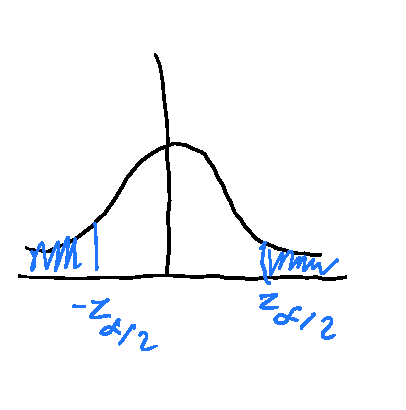
\includegraphics[width=.5\textwidth]{i2.pdf}

  Note that this is just for $\overline{X}_n$. What if we have
  something different?

  If $n$ is large and $\theta$ is a parameter of interest, then
  $$\frac{\hat{\theta}_n - \theta}{\sqrt{Var(\hat{\theta}_n)}} \stackrel{approx}{\sim}N(0,1)$$
  where $\hat{\theta}_n$ is an MLE (Maximum Likelihood Estimator,
  which we'll see in a future chapter)

  For example, if $X_i \sim Ber(p)$, i.e. $X_i =
  \begin{cases}
    1 & p \\ 0 & 1-p
  \end{cases}
  $ and $E(X_i) = p$, then $\overline{X}_n = \frac{1}{n}
  \sum_{i=1}^nX_i = \hat{p}_n$. So we want to estimate $\hat{p}_n$.
  \begin{flalign*}
    \frac{\hat{p}_n - p}{\sqrt{\frac{p(1-p)}{n}}}
    \sim N(0,1)
    \\ \hat{p}_n \pm 1.96 \sqrt{\frac{p(1-p)}{n}}
  \end{flalign*}
  But once again, we don't know what $p$ is and it is not useful! So
  we can either:
  \begin{itemize}
  \item Replace $p$ by $\hat{p}_n$
  \item Or, take the conservative approach and replace $p(1-p)$ by
    $\frac{1}{4}$ (remember that this is the max value the it can
    take, as seen earlier)
    \\ $f(x)=x(1-x) \to f'(x) = 1-2x = 0 \implies x=\frac{1}{2},
    f''(x)= -2, f(\frac{1}{2}) = \frac{1}{4}$, a max. Since we are
    replacing by the max, we are accounting for the worse situation,
    so it gives us a large confidence interval (which is why it is
    conservative). These are the types of intervals that we hear about
    before elections. When they are talking about chance they are
    talking about $\hat{p}_n$, when talking about how accurate it is,
    they are referring to the $\pm$ part and when saying it is right
    $19$ out of $20$ times, they are talking about the $\%$ of the CI.

    Now suppose we are interested in estimating the variance $\theta =
    p(1-p)$ (not interested in estimating $p$). What would be a
    natural estimator?
    \begin{flalign*}
      \hat{\theta}_n & = \hat{p}_n (1-\hat{p}_n)
      \\ \frac{\hat{\theta}_n - \theta}{\sqrt{Var(\hat{\theta}_n)}} & \sim N(0,1)
      \intertext{We then have the general recipe:}
      \hat{\theta}_n \pm Z_{\frac{\alpha}{2}}
      \sqrt{Var(\hat{\theta}_n)} \text{ is }100(1-\alpha)\% \text{ CI}
    \end{flalign*}
    The only thing we need is a right estimator that gives us this
    asymptotic normality and then we are in business! As long as our
    $\hat{\theta}_n$ can provide asymptotic normality for large $n$,
    then wen can have this. Most of the estimators in the textbook
    follow this pattern.
  \end{itemize}
  \noindent \rule{\textwidth}{0.5pt}
  \subsection{Small Sample Size} There are some cases we can solve and
  some that we cannot. The case of interest that we can solve, is the
  normal case. We are focusing a lot on normal distributions because
  we will see later that many things relate to the normal
  distribution, like comparing control groups on placebo and not on placebo.
  $X_i \stackrel{iid}{\sim} N(\mu, \sigma^2), i=1,\ldots,n$ where
  $n$ is ``small''. Here $\mu$ is of interest but $\sigma^2$ is a
  nuisance.
  
  We learned that $\frac{\overline{X}_n -
    \mu}{\frac{\sigma}{\sqrt{n}}} \stackrel{\text{Exact}}{\sim}
  N(0,1)$. So we can use this as a pivotal quantity to come up with a
  confidence interval for $\mu$. But we still have the $\sigma$ here
  that is a nuisance. Before we replaced $\sigma$ by $S$, but that was
  well justified because our sample size was large. But that's the
  best thing we have, so we'll use it. But can we say it is normally
  distributed? We were only able to say that earlier because we had a
  large distribution. So what might happen?
  $$\frac{\overline{X}_n - \mu}{\frac{S}{\sqrt{n}}} \sim T_{n-1}$$
  This will be similar to the $X_i$, i.e. normally distributed and it
  will still have a bell curve. But what about the tails? The
  uncertainty of $S$ means that the tails will die out more slowly.

  If $X_i \stackrel{iid}{\sim} N(\mu, \sigma^2), i=1,\ldots,n$, then
  $$\frac{\overline{X}_n - \mu}{\frac{S}{\sqrt{n}}} \sim T_{n-1}$$
  where $S^2 = \perp_{n-1} \sum_{i=1}^n (X_i - \overline{X}_n)$

  What is the $T$ distribution?
  $\frac{N(0,1)}{\sqrt{\frac{\chi^2_\nu}{\nu}}}$ where $N(0,1)
  \independent \chi^2_\nu$ and $\nu$ denotes the degrees of
  freedom. How does this relate to what we have?
  \begin{flalign*}
    \frac{(\overline{X}_n - \mu)}{\frac{\sigma}{\sqrt{n}}}/\left(\left(\frac{\sigma}{\sqrt{n}}\right)^{-1} \sqrt{\frac{S^2}{n}}\right) &
    \intertext{Where the numerator is }\sim N(0,1)
    \\ & = \frac{\frac{\overline{X}_n - \mu}{\frac{\sigma}{\sqrt{n}}}}{\sqrt{\frac{S^2}{\sigma^2}}}
  \end{flalign*}
  \begin{flalign*}
    \sqrt{\frac{S^2}{\sigma^2}} & = \sqrt{\frac{\sum_{i=1}^n \left(\frac{X_i - \overline{X}_n}{\sigma}\right)^2}{n-1}}
    \\ \sum_{i=1}^n \left( \frac{X_i - \overline{X_n}}{\sigma}\right)^2 & \sim \chi_{n-1}^2
  \end{flalign*}
  \section{01/30/18}
  \paragraph{Recall}
  When it comes to confidence intervals, the main tool is
  \textbf{pivotal quantities}. So whatever we did using large or small
  samples, was to come up with a pivotal quantity. In large samples,
  we used Central Limit Theorem. For small samples, the case that we
  studied assumed that observations came from a Normal distribution
  and so we used normality assumption in order to come up with a
  pivotal quantity. What happens when we go beyond Normal
  distribution? There is a general approach to get a pivotal quantity
  that covers all continuous random variables, but in practice it is
  only useful if we can find the distribution function of the variable
  of interest, but it is only useful if its easy to acquire. We will
  present the recipe today, which is sometimes successful and
  sometimes unsuccessful. Pivotal quantities are case by case, vary by
  distribution. This is already in the notes on myCourses:

  Say we have $X_1, \ldots, X_n \sim F (cdf) \to f (pdf)$. Suppose
  this is information from Revenue Canada and we made a histogram of
  the range of salaries and we fit a distribution over several years
  (this is our pdf). Now for this year, we'll be taking random people
  $(x_i)$ from Canada who have filled out their tax forms.

  Probability Integral Transform is a simple result that is very
  useful, especially in simulation. What it says is that if $X(\text{continuous}) \sim F
  \implies \underbrace{F(X)}_{Y} \sim Unif(0,1)$. I.e. apply $F$ on a
  continuous distribution and get another distribution, a uniform
  distribution on $(0,1)$. So how can we use this? If we can generate
  observations on a uniform distribution, then we can generate results for
  any continuous distribution by applying $F^{-1}$, (since $F$ is a
  monotone decreasing function it has an inverse) and then we get $X$s
  that are distributed like $X$, although uniform randomness is very
  difficult to achieve.

  \begin{flalign*}
    X \sim N(0,1)
    \\ f_X(x) & = \frac{1}{\sqrt{2 \pi}}e^{\frac{-x^2}{2}}, -\infty < x < + \infty
    \\ F_X(x) & = \int_{-\infty}^x f_x(t) \ dt = \int_{-\infty}^{x} \frac{1}{\sqrt{2\pi}}e^{-\frac{t^2}{2}} \ dt
    \intertext{This is a monotone function, but its inverse is very
      hard to find. What we do is generate uniform random numbers to
      approximate this and then get normal distribution. Try this at home:}
    X \sim F & Y = F(x)
    \intertext{You will see that the distribution of $Y$ is
      uniform. Use the method of transformation here (look in Chapter
      6). Now our result is:}
    X ~ F & \implies \underbrace{Y = F(X) \sim Unif(0,1)}_{PIT} \implies -2 \log Y \sim \chi^2_2
    \\ X_i \stackrel{iid}{\sim} F, & i=1,\ldots, n
    \\ Y_i & = F(X_i) \stackrel{iid}{\sim} Unif(0,1), i=1,2,\ldots,n
    \\ V_i & = -2 \log Y_i \stackrel{iid}{\sim} \chi_2^2, i=1,\ldots,n
    \\
  \end{flalign*}
  \begin{equation}
    \sum_{i=1}^nV_i \sim \chi_{2n}^2
  \end{equation}
    {This can easily be gotten to via the method of mgf. If
      $F$ has any unknown parameters, it will still be present in
      $V_i$. So $\sum_{i=1}^n V_i$ will depend on $X_i$s and
      parameters of $F$, but its distribution doesn't, so this is a
      pivotal quantity.}
  \paragraph{Ex} $X_i \stackrel{iid}{\sim} Exp(\lambda),
  i=1,2,\ldots,n$
  \begin{flalign*}
    f_X(x) & =
    \begin{cases}
      \lambda e^{-\lambda x} & x>0
      \\ 0 & x \leq 0
    \end{cases} \lambda >0
    \\ F_X(x) & = \int_{-\infty}^{x} f_X(t) \ dt = \int_0^x \lambda e ^{-\lambda t} \ dt
    \\ & = -e^{-\lambda t}|_0^x = 1-e^{-\lambda x}
  \end{flalign*}
  The dual to (3):
  \begin{flalign*}
    \sum_{i=1}^nW_i \sim \chi_{2n}^2
  \end{flalign*}
  where $W_i = -2 \log (1-Y_i)$. This is because, if $U \sim Unif
  (0,1)$ then $1-U \sim Unif(0,1)$. This is useful because we often
  want $1-F$, because the probability of $F$ is that something is less
  than something, so $1-F$ means that the value is past a certain
  point, i.e. this is good for the survivor function, checking the
  chances that someone survives past something.
  \begin{flalign*}
    F_X(x) & =
    \begin{cases}
      0 & \text{if }x \leq 0
      \\ 1-e^{-\lambda x} & \text{if }x>0
    \end{cases}
    \\ S_X(x) = 1-F_X(x) & =
    \begin{cases}
      1 & \text{if }x \leq 0
      \\ e^{-\lambda x} & \text{if }x>0
    \end{cases}
    \\ \sum_{i=1}^n W_i & = \sum_{i=1}^n - 2 \log [1-F(X_i)]
    \\ & = \sum_{i=1}^n - 2 \log e^{-\lambda X_i}
    \\ & = 2 \lambda \sum_{i=1}^n X_i = 2 \lambda n \overline{X}_n
    \\
    \\ 2 \lambda n \overline{X}_n & = \sum_{i=1}^n W_i \sim \chi_{2n}^2
  \end{flalign*}
  This is a pivotal quantity. So we can use this for a confidence
  interval of lambda.

  Using the $\chi^2$ table (Appendix 3, p850-851), we can find:
  \begin{flalign*}
    \chi_{2n,0.025}^2 \& \chi_{2n, 0.975}^2
    \\ P \left(\chi_{2n,0.975}^2 < 2 \lambda n \overline{X}_n < \chi_{2n,0.025}^2\right) & = 95\% = 0.95
    \\ P \left(\frac{\chi_{2n,0.975}^2}{2 n \overline{X}_n} < \lambda < \frac{\chi_{2n,0.025}^2}{2 n \overline{X}_n}\right) & = 95\% = 0.95
  \end{flalign*}
  So: $ \left(\frac{\chi_{2n,0.975}^2}{2n \overline{X}_n} ,
    \frac{\chi_{2n, 0.025}}{2 n \overline{X}_n}\right)$ is a $95\%$
  C.I. for $\lambda.$
  \\ 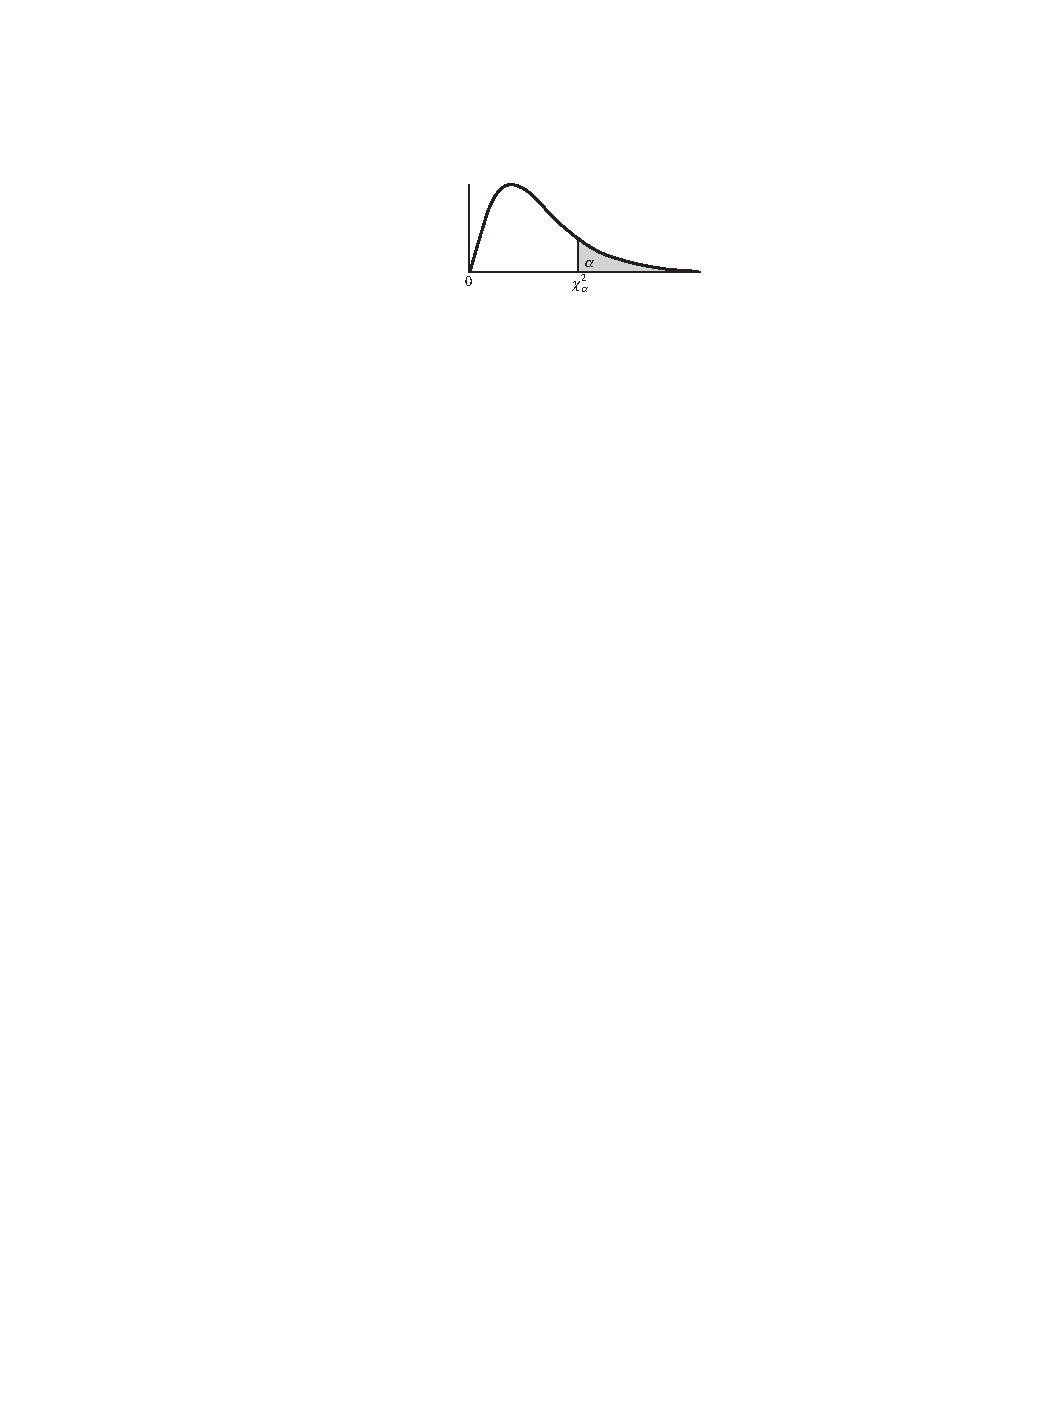
\includegraphics[width=.9\textwidth]{i3.pdf}
  \subsection{Sample Size Determination} Say we want to predict the
  results of an election. We want to be, say $99\%$ sure of the
  results (why not $100\%$? because then we'd need infinite samples).

  \begin{flalign*}
    X_i & =
    \begin{cases}
      1 & \text{NDP}
      \\ 0 & \text{otherwise}
    \end{cases}
    , i=1,\ldots,n
    \\ p(X_i = 1) & = p
    \\ X_i \stackrel{iid}{\sim} & Bernoulli(p), i=1,\ldots,n
    \\ \hat{p}_n & = \frac{1}{n} \sum_{i=1}^n X_i
    \intertext{We want $|\hat{p}_n - p| \leq 0.01$ with $95\%$. We
      can use Chebyshev's for this, but since Chebyshev's makes very
      little assumptions, the bound is very crude. We want a tighter
      bound. So we can use CLT: }
    \hat{p}_n \pm \underbrace{1.96 \sqrt{\frac{p(1-p)}{n}}}_{B}
    \intertext{This is called a symmetric confidence interval, since
      it is centered around a point. Normal distribution is symmetric,
    $\chi$ is not. If it is symmetric, we can talk about length or
    half length, if it isn't we talk about the whole length.}
     \text{(e.g. 0.01)} \to B & = 1.96 \sqrt{\frac{p(1-p)}{n}}
    \intertext{Say we want it in terms of $100(1-\alpha)\%$:}
    B & = Z_{\frac{\alpha}{`2}} \sqrt{\frac{p(1-p)}{n}}
  \end{flalign*}
  We obtain:
  \begin{equation*}
    n = \frac{p(1-p)(Z_{\frac{\alpha}{2}})^2}{B^2}
  \end{equation*}
  We have the following 2 options:
  \begin{itemize}
  \item Replace $p$ by $\hat{p}_n$ (a prior estimate, although often
    we don't have an estimate).
  \item Replace $p(1-p)$ by $\frac{1}{4}$ (conservative approach).
  \end{itemize}
  So then we get:
  \begin{equation*}
    n = \frac{Z_{\frac{\alpha}{2}}^2}{4B^2}
  \end{equation*}
  (we round up $n$ if it is not an integer) This gives us a sample
  size! This is a proportion estimate for the sample size for Bernoulli.
  \paragraph{Ex} $B=0.01, \alpha = 0.05$
  \begin{flalign*}
    n & = \frac{(1.96)^2}{4(0.01)^2} =9604 \approx 10,000
  \end{flalign*}
  \\ \noindent \rule{\textwidth}{0.5pt}
  Now, generalizing:

  C.I. for $\mu$:
  \begin{flalign*}
    \overline{X}_n \pm \underbrace{Z_{\frac{\alpha}{2}} \frac{\sigma}{\sqrt{n}}}_{B}
    \\ B & = Z_{\frac{\alpha}{2}} \frac{\sigma}{\sqrt{n}}
    \\ n & = \frac{Z_{\frac{\alpha}{2}}^2 \sigma^2}{B^2} \text{ for }\mu
  \end{flalign*}
  Here we can't just maximize $\sigma$, so we do pilot studies, where
  we try to justify the need for a study, so we receive a little bit
  of money to make a small study, to get an idea of some of the
  parameters, like $\sigma$ in this case and then we use this
  parameter to get a bit of information on other parameters so that we
  can apply for the real study. Now determining the sample size goes
  back to confidence intervals.
  \\ \noindent \rule{\textwidth}{0.5pt}
  Other variables:
  \begin{equation}
    \frac{\hat{\theta}_n - \theta }{\sqrt{Var(\hat{\theta}_n)}}
    \stackrel{app}{\sim} N (0,1) \text{ for large }n
  \end{equation}
  Here $\hat{\theta}_n$ is the MLE (will see in the future) and
  $\theta$ is the estimand.
  \begin{flalign*}
    \hat{\theta}_n \pm Z_{\frac{\alpha}{2}} \sqrt{Var(\hat{\theta}_n)}
    \intertext{$100(1-\alpha)\%$ C.I. for $\theta$}
    B = Z_{\frac{\alpha}{2}} \sqrt{Var(\hat{\theta}_n)}
  \end{flalign*}
  So we get:
  \begin{itemize}
  \item Bernoulli $Var(\hat{\theta}_n) = \frac{p(1-p)}{n}$
  \item $\mu$ $Var(\overline{X}_n) = \frac{\sigma^2}{n}$
  \end{itemize}
  These are based on a large sample. What if we have a small sample
  size? As long as we have the confidence interval, if it is symmetric
  we can bound by half length, if it isn't we can bound by the whole
  length.

  Normal case:
  \begin{flalign*}
    \overline{X}_n \pm t_{\frac{\alpha}{2}, (n-1)} \frac{\sigma}{\sqrt{}}
    \\ B = t_{\frac{\alpha}{2}, (n-1)} \frac{s}{\sqrt{n}}
  \end{flalign*}
  \\ \noindent \rule{\textwidth}{0.5pt}
  So far we've talked about one population. So what happens if we have
  two populations? Say we have men and women and want to estimate
  average salary.
  \begin{flalign*}
    \frac{\hat{\theta}_n - \theta}{\sqrt{Var(\hat{\theta}_n)}} \sim N(0,1)
  \end{flalign*}
  How do we use this if we have more than one sample, say $X_1,
  \ldots, X_m$ (men, $\overline{X}_m$) and $Y_1, \ldots, Y_n$ (women, $
  \overline{Y}_n$). Say we want to estimate $\theta = \mu_M -
  \mu_W$. Then $\hat{\theta} = \overline{X}_m - \overline{Y}_n$. Now,
  using the formula above, we get:
  \begin{flalign*}
    \frac{(\overline{X}_m - \overline{Y}_m) - (\mu_M - \mu_W)}{\sqrt{Var(\overline{X}_m - \overline{Y}_m)}}
  \end{flalign*}
  So the general recipe is:
  
  Pivotal quantity -> confidence interval -> margin of error -> sample
  size

  \begin{flalign*}
    Var(\overline{X}_m - \overline{Y}_n) & = Var(\overline{X}_m) + Var(\overline{Y}_n) - 2Cov(\overline{X}_m, \overline{Y}_n)
    \intertext{Assuming that $X$s \& $Y$s are independent (note that
      we don't need independence, just orthogonality such that $Cov$
      is $0$, independence is much stronger). Then $Cov(\overline{X}_m
      , \overline{Y}_n) = 0$}
    Var(\overline{X}_m - \overline{Y}_n) & = Var(\overline{X}_n) + Var(\overline{Y}_n) = \frac{\sigma_M^2}{m} + \frac{\sigma_W^2}{n}
    \\ \frac{(\overline{X}_m - \overline{Y}_n) - (\mu_M -
      \mu_W)}{\sqrt{\frac{\sigma_M^2}{m}}+ \frac{\sigma_W^2}{n}}
    \stackrel{approx}{\sim} N(0,1) \text{ for large }m \& n
    \\ (\overline{X}_m - \overline{Y}_n) & \pm Z_{\frac{\alpha}{2}} \sqrt{\frac{\sigma_M^2}{m}+ \frac{\sigma_W^2}{n}}
      \intertext{is a $100(1-\alpha)\%$ C.I. for $\mu_M-\mu_w$}
      B & = Z_{\frac{\alpha}{2}} \sqrt{\frac{\sigma_M^2}{m}+ \frac{\sigma_W^2}{n}}
        \\ \left(\frac{B}{Z_{\frac{\alpha}{2}}}\right)^2 & = \frac{\sigma_M^2}{m} + \frac{\sigma_W^2}{n}
        \intertext{So we have one equation with $2$ unknowns. What
          should we do? Set them equal! What is the rational for
          setting them equal? Cost. If $u=km$, we can solve:}
        \left(\frac{B}{Z_{\frac{\alpha}{2}}}\right)^2 & = \frac{1}{m} \left(\sigma_M^2 + \frac{\sigma_W^2}{k}\right)
        \\ m & = \frac{\sigma_M^2 + \frac{\sigma^2_W}{k}} {\left(\frac{B}{Z_{\frac{\alpha}{2}}}\right)^2}
  \end{flalign*}
  With proportions $\sigma_M^2 = p_M(1-p_M)$ can replace with
  $\frac{1}{u}$, much simpler:
  $$\rightarrow \frac{1+\frac{1}{k}}{ \left(\frac{B}{Z_{\frac{\alpha}{2}}}\right)^2}$$
\end{document}